\linespread{1.5}

\textbf{Solução}

\textbf{a)}
\begin{equation*}
    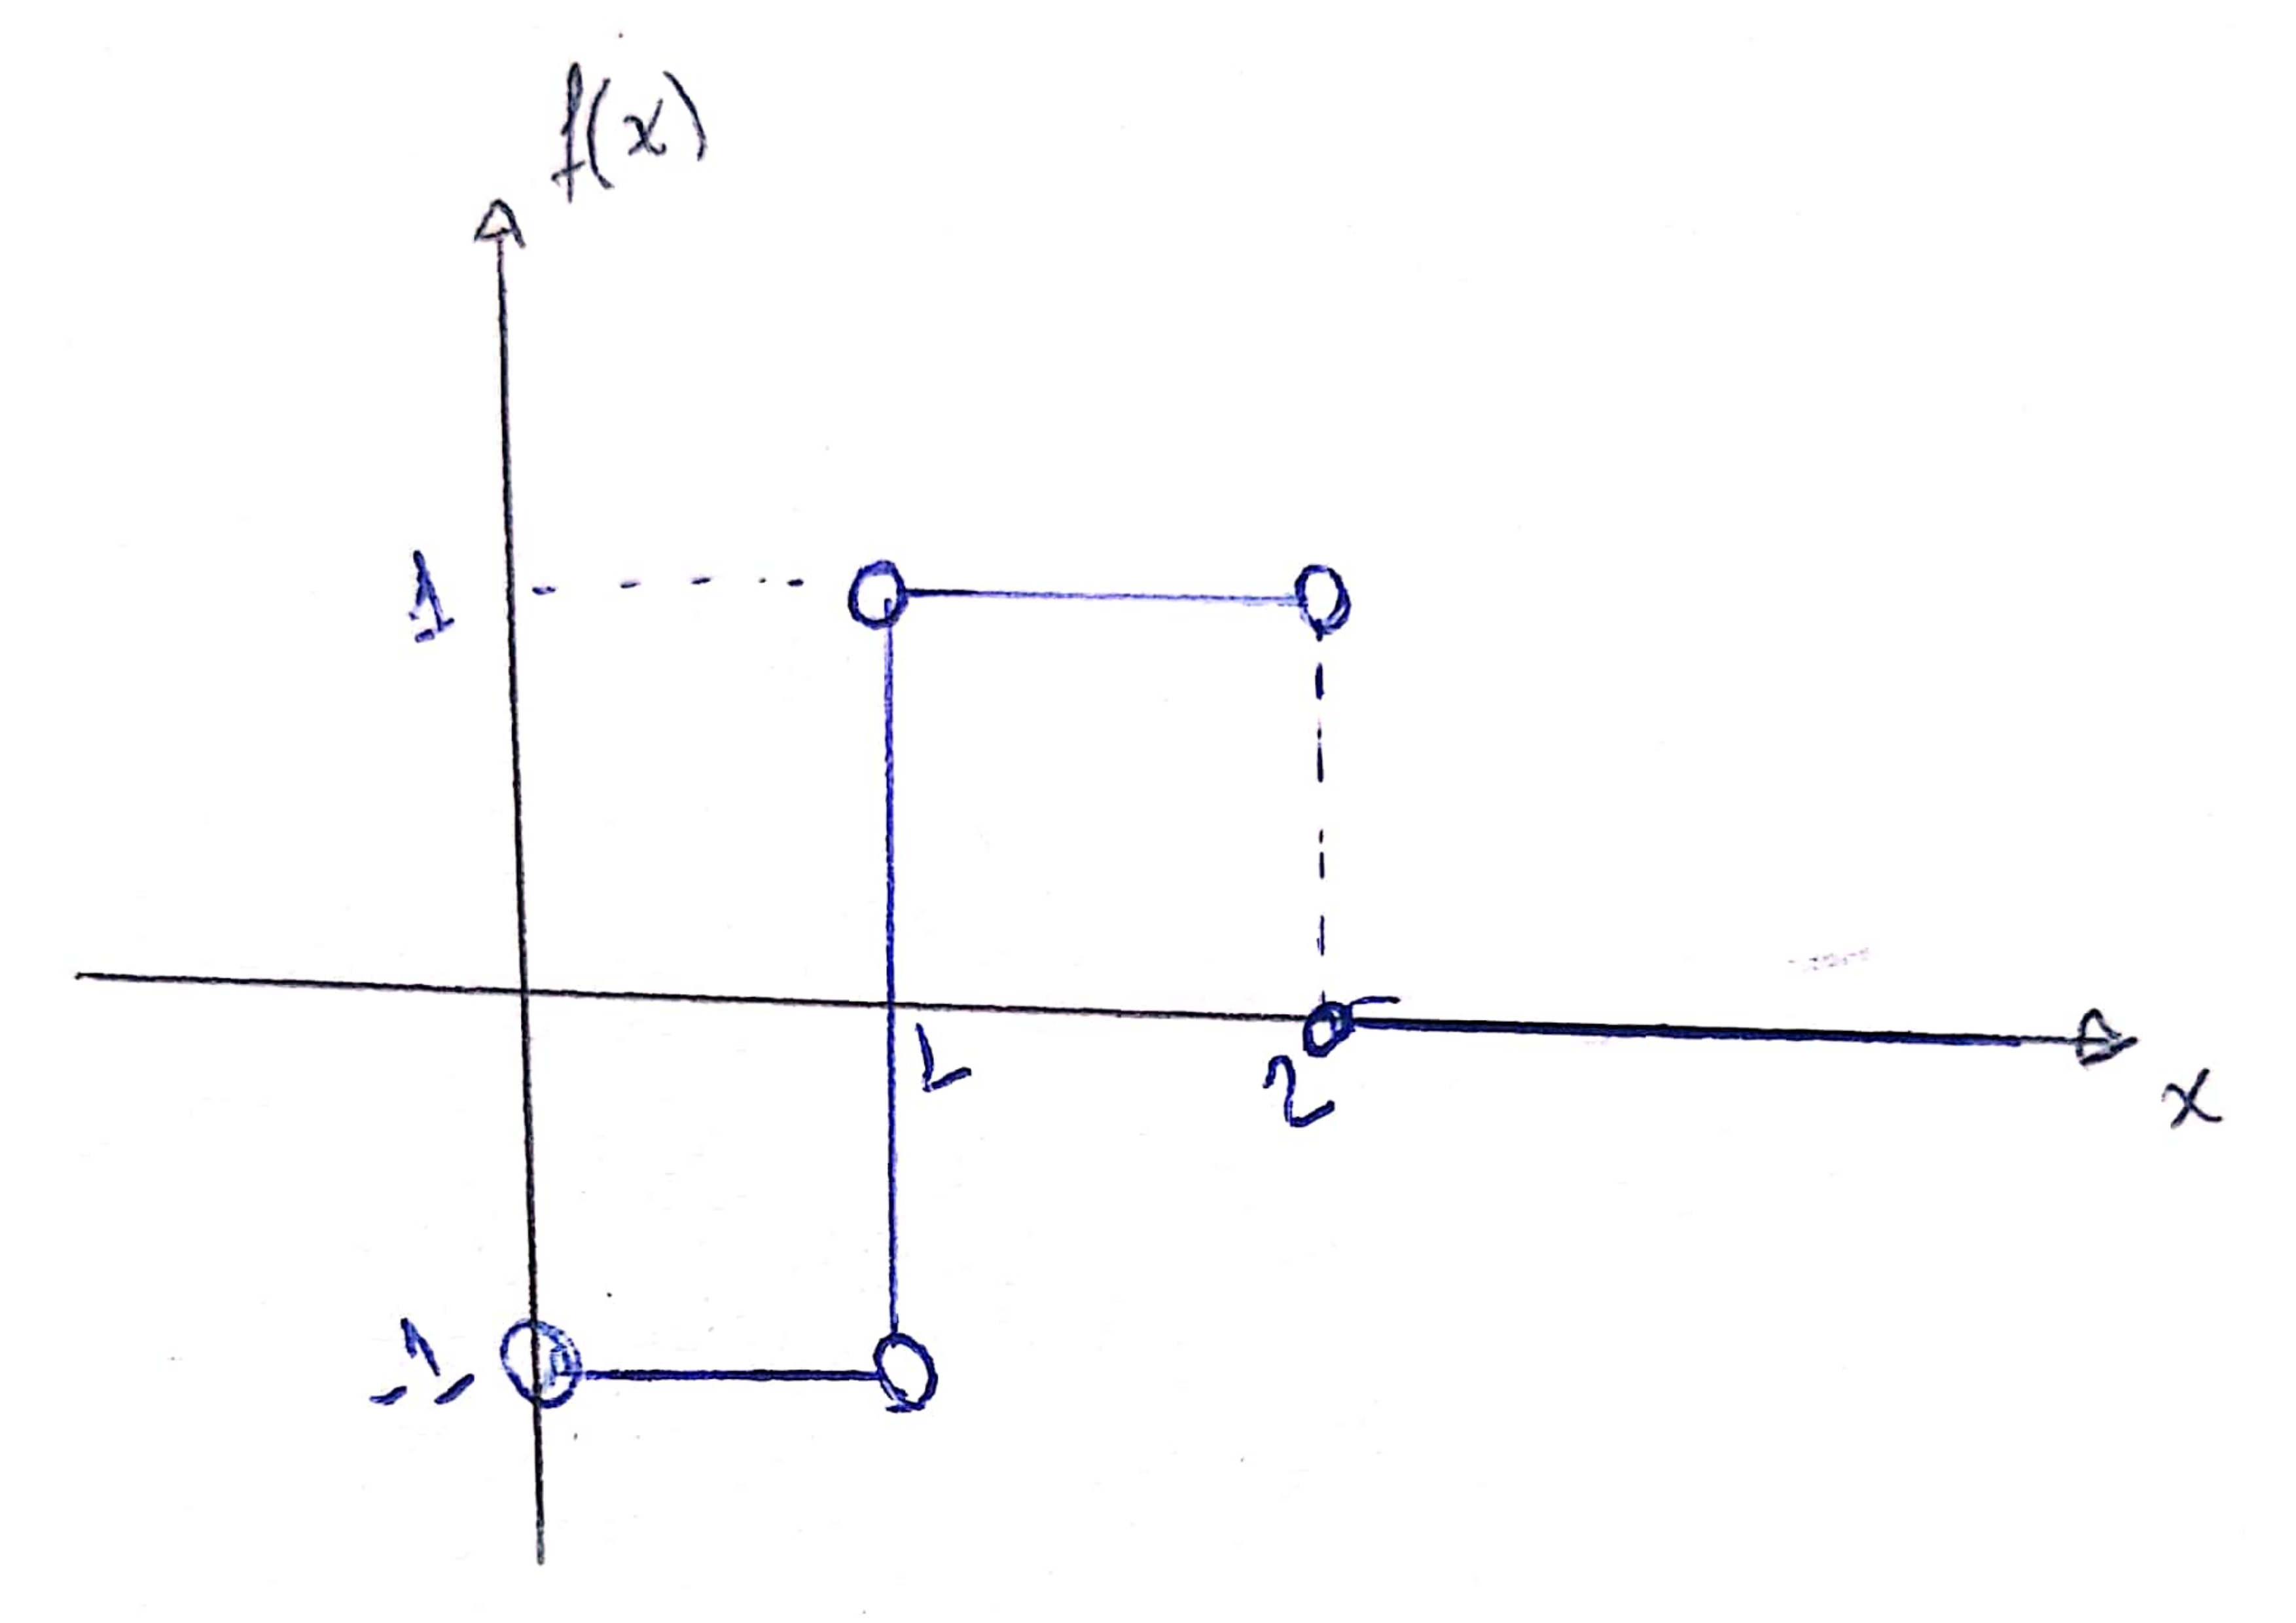
\includegraphics[width = 0.5\linewidth]{fig/tf2a.png}
\end{equation*}


\textbf{b)} Como a função $f(x)$ atende aos critérios do Teorema de Fourier, então a transformada de Fourier cosseno pode ser calculada da seguinte forma:
\begin{equation*}
    \hat{f_c}(w) = \sqrt{\frac{2}{\pi}}\int_0^\infty f(x)cos(wx)dx
\end{equation*}
\begin{equation*}
    \hat{f_c}(w) = \sqrt{\frac{2}{\pi}}\left[\int_0^1 -cos(wx)dx + \int_1^2 cos(wx)dx\right] =  \sqrt{\frac{2}{\pi}}\left\{\left[\frac{-\sin(wx)}{w} \right]_0^1 + \left[\frac{sin(wx)}{w}\right]_1^2\right\}
\end{equation*}
\begin{equation*}
    = \sqrt{\frac{2}{\pi}}\left\{\left[\frac{-\sin(w)}{w} \right] + \left[\frac{sin(2w)}{w} - \frac{-sin(w)}{w}\right]_1^2\right\} \therefore \boxed{\hat{f_c}(w) =  \sqrt{\frac{2}{\pi}} \left(\frac{sin(2w) - 2sin(2w)}{w}\right)}
\end{equation*}
